The radiation damage created by \ac{HL-LHC} will become a big challenge for the innermost 
\begin{figure}[h]
	\centering
	\subfig[.43]{PlanarConcept.png}{.2}{planar}
	\begin{subfigure}{0.1\textwidth}  
		\centering 
		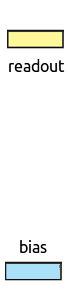
\includegraphics[height=.2\textheight]{LegendConcept.png}
		\vspace*{19pt}
	\end{subfigure}
	\subfig[.43]{3DConcept.png}{.2}{3D}
	\caption{Comparison of the planar and the 3D detector concepts}
	\label{3d1}
\end{figure}
\noindent tracking detectors. After a large irradiation, all detector material will become trap limited with a \ac{MFP} below \SI{75}{\micro\meter}. The concept of a so called 3D-Detector is a possible way to highly increase the longevity of these materials. Its basic principle is shown in figure \vref{3d1}: In a planer detector the readout and bias electrodes are brought onto the front and back side of the sensor with a thickness $\Updelta$. The resulting drift distance L of the charge carriers is of the order of $\Updelta$. In the 3D detector the electrodes are put inside of the detector material so that the \acp{MIP} can travel the same distance $\Updelta$ in the material and therefore create the same amount charge carriers but L is heavily reduced. In case of diamond these electrode columns are drilled with a \SI{800}{\nano\meter} femtosecond laser which converts the diamond into a resistive mixture of carbon phases.\\
In 2015 one of the first detectors was built out of a \ac{pCVD} diamond sensor which had a 3D detector 
\wrapfigcl{3DMultiResult.png}{.3}{Pulse height of the 3D multi detector}{3d2}
as well as a strip detector on the same sensor. At this time the column efficiency was about \SI{92}{\%} and the 3D cells had a size of \SI{150x150}{\micro\meter}. This detector was already a success by showing a working 3D diamond detector. Its square cells are clearly visible and the measured signal for the thickness of \SI{500}{\micro\meter} was \SI{13500}{e} which is much higher than \SI{6900}{e} in the strip detector. The strip signal equates to a \ac{CCD} of \SI{192}{\micro\meter}. The measured charge in the 3D would have a \ac{CCD} in a planar detector of \SIrange{350}{375}{\micro\meter} which effectively means that more than \SI{75}{\%} of the created charge was collected for the 
first time in a \ac{pCVD} diamond. The according pulse height distributions are shown in figure \vref{3d2}.\\
The next step followed in 2016 when the full 3D detectors was built was dramatic improvements. The number of cells went up from 99 to 1188, the cell size was reduced to to \SI{100x100}{\micro\meter} and the column efficiency could be increased to \SI{99}{\%}. The analysis of this device is still in progress but the first results already look very promising. There is charge in the entire area of the detector and we see the largest charge collection in \ac{pCVD} yet with over \SI{85}{\%} in a contiguous region.\\
Finally in the end of 2016 the first \ac{pCVD} 3D pixel detector was built. A 3D diamond sensor was metallised and then bump bonded to a CMS pixel \ac{ROC} psi46v2.1respin. The chip was then tuned to a global pixel threshold of \SI{1500}{e}. The preliminary beam test results already look very with an efficiency of \SI{98.5}{\%}. This value is close to the efficiency of the silicon pixel of \SI{99.3}{\%} which was tested in parallel. The slightly lower value is believed to origin from the low field regions between the electrodes.